% !TeX root = ../index.tex

\section{Technische Anforderungen und Systemdesign}

\subsection{Technische Anforderungen}
Nachfolgend werden die technischen Anforderungen an das \gls{iot}-System beschrieben.

\paragraph{Systemübersicht}
Die \gls{iot}-Gartenbewässerungsanlage sollte in der Lage sein, den Wasserverbrauch effizient und automatisch zu steuern, um den Pflanzen im Garten eine optimale Bewässerung zu bieten. Das System sollte aus Sensoren, Aktoren, einer zentralen Steuereinheit und einer Benutzeroberfläche bestehen.

\paragraph{Sensoren}
\begin{itemize}
  \item Boden-Feuchtigkeitssensoren: zur Messung der aktuellen Bodenfeuchtigkeit in verschiedenen Bereichen des Gartens
  \item Boden-Temperatursensoren: zur Messung der aktuellen Bodentemperatur in verschiedenen Bereichen des Gartens
  \item Luft-Feuchtigkeitssensor: zur Erfassung der aktuellen Feuchtigkeit in der Luft
  \item Luft-Temperatursensor: zur Erfassung der aktuellen Umgebungstemperatur in der Luft
  \item Lichtsensor: zur Erfassung der aktuellen Sonneneinstrahlung
\end{itemize}

\paragraph{Aktoren}
\begin{itemize}
  \item Wasserpumpe: zur Beförderung des Wassers aus einer Wasserquelle (z.B. Regenwasserzisterne) in das zu bewässernde Beet
  \item Sonnenschutz: zum Schutz von lichtempfindlichen Pflanzen bei zu starker Sonneneinstrahlung
\end{itemize}

\paragraph{Stromversorgung}
\begin{itemize}
  \item Anschluss an Netzstrom: standardmäßig wird davon ausgegangen, dass das zu bewässernde Gartenbeet Anschluss an den Netzstrom hat
  \item alternative Energiequellen: Solarzellen und/oder Batterien, falls keine Versorgung über Netzstrom möglich ist
\end{itemize}

\paragraph{Kommunikation}
\begin{itemize}
  \item Mikrocontroller: zur Verarbeitung der Sensordaten, Steuerung der Aktoren und Kommunikation über eine Netzwerkschicht
  \item Kommunikationsprotokoll: \gls{wlan}, um eine drahtlose Verbindung zwischen den Hardwarekomponenten und der Steuereinheit herzustellen
\end{itemize}

\paragraph{Steuereinheit}
\begin{itemize}
  \item Zentraler Server: Steuerung der \gls{iot}-Gartenbewässerungsanlage auf Basis selbst implementierter Funktionslogik
\end{itemize}

\paragraph{Benutzeroberfläche}
\begin{itemize}
  \item Smartphone-App oder Webanwendung: zur Fernsteuerung und Überwachung der \gls{iot}-Gartenbewässerungsanlage, Anzeige von Sensordaten und Einstellung von Bewässerungsparametern
  \item Benachrichtigungsfunktion: um den Benutzer über den aktuellen Systemstatus oder wichtige Ereignisse (z.B. Frostgefahr) zu informieren
\end{itemize}

\paragraph{Softwareanforderungen}
\begin{itemize}
  \item Automatisierung: Die Bewässerungsanlage sollte in der Lage sein, automatisch auf Basis der Sensordaten und vordefinierter Schwellenwerte zu arbeiten
  \item Manueller Modus: Möglichkeit zur manuellen Steuerung der Bewässerung über die Benutzeroberfläche, falls erforderlich
  \item Anpassungsfähigkeit: Die Software sollte in der Lage sein, mit unterschiedlichen Gartenlayouts, Pflanzentypen und Bewässerungszonen umzugehen
\end{itemize}


\subsection{Aufbau der Systemarchitektur}

Für die Umsetzung der technischen Anforderungen wird die in in Abb. \ref{fig:iotschichten} modellierte Systemarchitektur gewählt.

\begin{figure}[h]
  \centering
  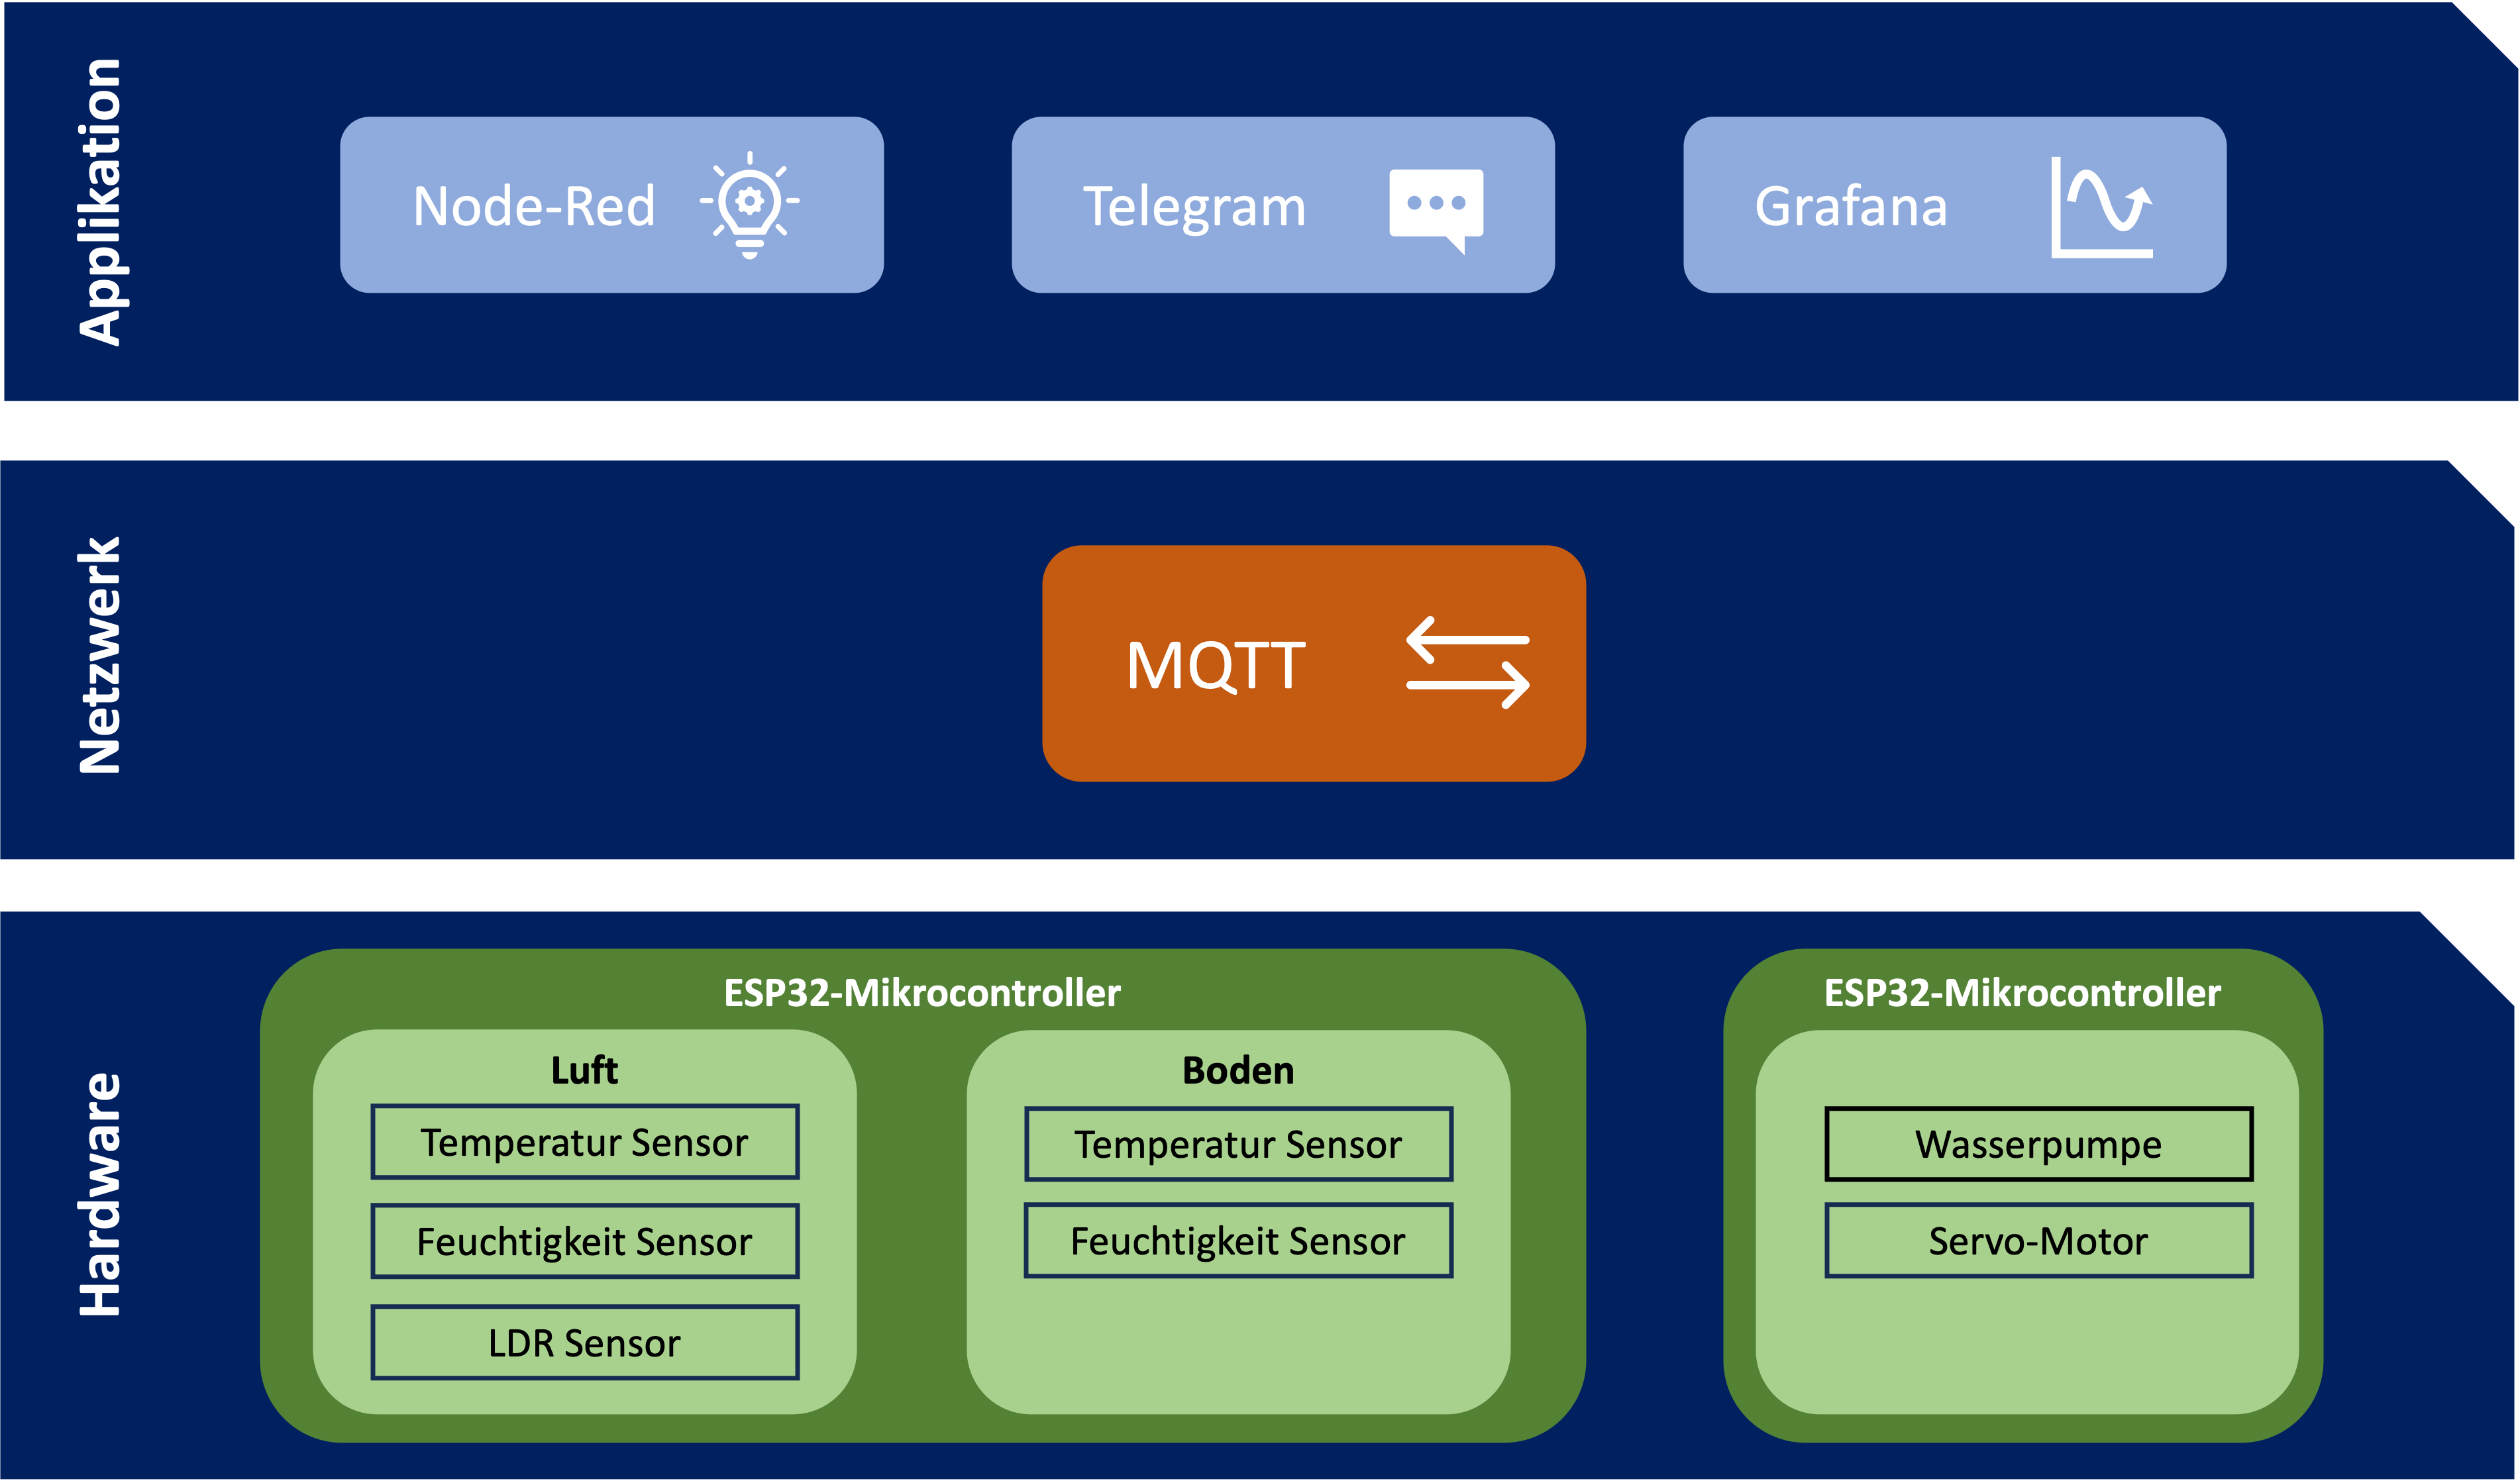
\includegraphics[width=0.8\textwidth]{Aufbau_Architektur.png}
  \caption{Aufbau der IoT-Architektur}\label{fig:iotschichten}
\end{figure}

Auf Hardwareebene kommt ein ESP32-Mikrocontroller zum Einsatz, um die Sensordaten über einen MQTT-Broker zu veröffentlichen. Gleichzeitig wird für die Aktoren ein eigener ESP32-Mikrocontroller eingesetzt, um die Wasserpumpe und Beschattung über eine Markise mit Servo-Motor zu steuern. Die Befehle zur Steuerung der Aktoren werden von dem MQTT-Broker empfangen. Der MQTT-Broker agiert dabei als Vermittler der Nachrichten in der Netzwerkschicht. In der Applikationsschicht wird mit Node-RED die Logik für die \gls{iot}-Steuerung implementiert, über Telegram werden der Benutzer über wichtige Informationen benachrichtigt und in Grafana werden mittels eines Dashboards relevante Daten in Form von Auswertungen für den Nutzer aufbereitet.

Die einzelnen Schichten aus der Systemarchitektur werden in den nachfolgenden Kapiteln näher beschrieben.